% !TEX root= ../main.tex
\documentclass[main.tex]{subfiles}

\begin{document}
\section{PRINCIP TERMONUKLEÁRNÍ FÚZE}
\subsection{Fyzika jaderné fúze}

\lipsum[3]~\cite{hejzlar}

\lipsum[2-4]
\subsection{Lorem ipsum}
\lipsum[1]

\begin{figure}[]
    \centering
    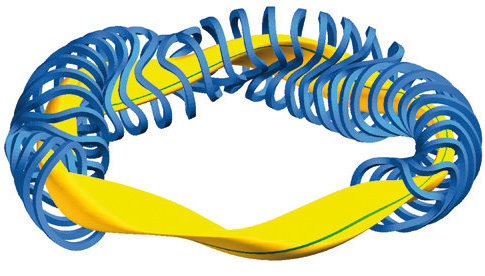
\includegraphics[width=0.6\textwidth]{obrazky/stelarator.jpg}
    \caption{Magnetické cívky a plazma stelarátoru Wendelstein 7-X.\cite{wx-7}}
    \label{fig:wx-7}
\end{figure}
\lipsum[1]
\(F=a^2\)
\begin{table}[]
    \centering
    \caption{Parametry pohonu pro 100 MW CBFR-SPS.~\cite{cheung2004colliding}}
    \begin{tabular}{  p{19em}  p{3em}  p{3em}  p{3em}  }
                                               & D-T  & D-He & H-B \\ \toprule
    Specifický impuls \(I_{sp}\times10^6\) (s) & 1.3  & 1.4  & 1.4 \\
    Výkon v tahu, \(P_T\) (MW)                 & 29.9 & 67.8 & 50.8 \\
    \(P_T/P_0\)                                & 0.3  & 0.68 & 0.51 \\
    Tah,\(T\) (N)                              & 3.8  & 9.6  & 28.1 \\
    \(T/P_0\) (mN/MW)                          & 37.8 & 95.5 & 281 \\ \bottomrule
    \end{tabular}
    \label{tab:cbfrsps}
\end{table}
\FloatBarrier
\end{document}